% %TC:ignore

% % \documentclass[14pt]{article}
% % \documentclass{book}
% % \documentclass[12pt, a4]{article}
% \documentclass[12pt, a4]{book}
% \linespread{1.5}
% % Engine-specific settings
% % Detect pdftex/xetex/luatex, and load appropriate font packages.
% % This is inspired by the approach in the iftex package.
% % pdftex:
% \ifx\pdfmatch\undefined
% \else
%     \usepackage[T1]{fontenc}
%     \usepackage[utf8]{inputenc}
% \fi
% % xetex:
% \ifx\XeTeXinterchartoks\undefined
% \else
%     \usepackage{fontspec}
%     \defaultfontfeatures{Ligatures=TeX}
% \fi
% % luatex:
% \ifx\directlua\undefined
% \else
%     \usepackage{fontspec}
% \fi
% % End engine-specific settings

% \usepackage{amsmath,amssymb}
% \usepackage{fullpage}

% \usepackage{graphicx,wrapfig,lipsum}
% \usepackage[svgnames, dvipsnames]{xcolor}
% \usepackage{url}
% \urlstyle{same}

% \usepackage[makestderr]{pythontex}
% \restartpythontexsession{\thesection}


% \usepackage[framemethod=TikZ]{mdframed}

% \newcommand{\pytex}{Python\TeX}
% % \renewcommand*{\thefootnote}{\fnsymbol{footnote}}

% \usepackage[comma,authoryear,round]{natbib}
% \usepackage{usebib}
% \bibliographystyle{apsr}


% % \usepackage{biblatex}
% % \usepackage[
% % backend=biber,
% % style=alphabetic,
% % sorting=ynt
% % ]{biblatex}
% % \addbibresource{MyLibrary.bib}
% % \usepackage{harvard}
% % \newbibfield{editor}
% % \bibinput{\jobname}

% % \bibliographystyle{abbrvnat}

% % \setcitestyle{authoryear} %Citation-related commands
% % \setcitestyle{citesep={;}, aysep={,}}


% % \usepackage[dvipsnames]{xcolor}

% \graphicspath{{images/}}
% %
% % \usepackage{mathptmx}      % use Times fonts if available on your TeX system
% %
% % insert here the call for the packages your document requires
% \usepackage{latexsym}
% \usepackage{hyperref} 
% \usepackage{mathtools}
% \usepackage{calculator}
% \usepackage{longtable}
% \usepackage{booktabs}

% \usepackage{siunitx}
% \usepackage{url}
% \sisetup{round-mode=places,round-precision=0}

% \usepackage{pgfplots}
% \usepgfplotslibrary{polar}
% \usepgflibrary{shapes.geometric}
% \usetikzlibrary{calc}
% \pgfplotsset{my style/.append style={axis x line=middle, axis y line=middle, xlabel={$x$}, ylabel={$y$}, axis equal }}

% % graphicx latexsym hyperref mathtools amssymb siunitx url

% % \smartqed  % flush right qed marks, e.g. at end of proof
% \RequirePackage{fix-cm}
% \usepackage{enumerate}
% \usepackage{manfnt}
% \usepackage{tikz-cd}
% \usetikzlibrary{automata, positioning, arrows}
% \usetikzlibrary{decorations.pathreplacing,positioning, arrows.meta}

% \usepackage{tabularx,ragged2e}
% \newcolumntype{C}{>{\Centering\arraybackslash\hspace{0pt}}X}
% \newcolumntype{Y}{>{\RaggedRight\arraybackslash\hspace{0pt}}X}

% \usepackage{color}
% \hypersetup{
%     linktoc=black, % 'all' will create links for everything in the TOC
%     colorlinks=true,
%     linkcolor=black,
%     filecolor=magenta,
%     urlcolor=black,
%     pdftitle={Sharelatex Example},
%     bookmarks=true,
%     pdfpagemode=FullScreen,
%     citecolor=black
% }

% \definecolor{aliceblue}{HTML}{00F9DE}

% \usepackage{amsfonts}
% \usepackage{bondgraphs}
% \usepackage{xfrac}
% \usepackage[normalem]{ulem}

% % \usepackage{slashbox}
% \usepackage{diagbox}

% \usepackage{multicol}

% \usepackage{ifthen}
% \newboolean{firstanswerofthechapter}  


% \colorlet{lightcyan}{cyan!40!white}

% \usepackage{chngcntr}
% \usepackage{stackengine}
% \usepackage{rotating}

% \usepackage{tasks}
% \newlength{\longestlabel}
% \settowidth{\longestlabel}{\bfseries viii.}
% \settasks{label=\roman*., label-format={\bfseries}, label-width=\longestlabel,
% item-indent=0pt, label-offset=2pt, column-sep={10pt}}

% \usepackage[lastexercise,answerdelayed]{exercise}
% \counterwithin{Exercise}{chapter}
% \counterwithin{Answer}{chapter}
% \counterwithin{Solution}{chapter}

% \renewcounter{Exercise}[chapter]
% \newcommand{\QuestionNB}{\bfseries\arabic{Question}.\ }

% \renewcommand{\ExerciseName}{Puzzle}
% \renewcommand{\ExerciseHeader}{\def\stackalignment{l}% code from https://tex.stackexchange.com/a/195118/101651
%     \stackunder[0pt]{\colorbox{cyan}{\textcolor{white}{\textbf{\LARGE\ExerciseHeaderNB\;\large\ExerciseName}}}}{\textcolor{lightcyan}{\rule{\linewidth}{2pt}}}\medskip}

% \newcounter{Puzzle}
% \newenvironment{Puzzle}{\begin{Exercise}[name={Puzzle},
% counter={Puzzle}]}
% {\end{Exercise}}


% \renewcommand{\AnswerName}{Exercises}
% \renewcommand{\AnswerHeader}{\ifthenelse{\boolean{firstanswerofthechapter}}%
%     {\bigskip\noindent\textcolor{cyan}{\textbf{CHAPTER \thechapter}}\newline\newline%
%         \noindent\bfseries\emph{\textcolor{cyan}{\AnswerName\ \ExerciseHeaderNB, page %
%                 \pageref{\AnswerRef}}}\smallskip}
%     {\noindent\bfseries\emph{\textcolor{cyan}{\AnswerName\ \ExerciseHeaderNB, page \pageref{\AnswerRef}}}\smallskip}}
% \renewcommand{\AnswerName}{Exercises}
% \renewcommand{\AnswerHeader}{\ifthenelse{\boolean{firstanswerofthechapter}}%
%     {\bigskip\noindent\textcolor{cyan}{\textbf{CHAPTER \thechapter}}\newline\newline%
%         \noindent\bfseries\emph{\textcolor{cyan}{\AnswerName\ \ExerciseHeaderNB, page %
%                 \pageref{\AnswerRef}}}\smallskip}
%     {\noindent\bfseries\emph{\textcolor{cyan}{\AnswerName\ \ExerciseHeaderNB, page \pageref{\AnswerRef}}}\smallskip}} 
    
% \setlength{\QuestionIndent}{16pt}

% % \usepackage{caption}
% \usepackage{float} % USED TO FORCE IMAGES INLINE
% \usepackage{subcaption}
% \usepackage{geometry}
% \usepackage{pdflscape}
% % \geometry{margin=1.8in}
% % \usepackage[a4paper, total={6in, 8in}]{geometry}
% % \geometry{margin=1.3in}
% % \linespread{1.3}

% \geometry{margin=1.4in}
% \linespread{1.1}

% \pagenumbering{gobble}
% \usepackage{verbatim}
% \immediate\write18{texcount -tex -sum  \jobname.tex > \jobname.wordcount.tex}

% % Keywords command
% \providecommand{\keywords}[1]
% {
%   \small	
%   \textbf{\textit{Keywords---}} #1
% }

% % \usepackage{xcolor}     % for colour
% % \usepackage{lipsum}     % for sample text
% \usepackage{ntheorem}   % for theorem-like environments
% % \usepackage{mdframed}   % for framing

% \theoremstyle{break}
% \theoremheaderfont{\bfseries}

% \newmdtheoremenv[%
% linecolor=gray,
% leftmargin=60,%
% rightmargin=60,
% backgroundcolor=gray!40,%
% innertopmargin=10,%
% ntheorem]{puzzle}{Puzzle}[section]

% \newmdtheoremenv[%
% linecolor=gray,
% leftmargin=60,%
% rightmargin=60,
% backgroundcolor=gray!7,%
% innertopmargin=10,%
% ntheorem]{solution}{Solution}[section]



% % \newcommand{\mpp}{\textsc{\textbf{mpp}}}
% % \newcommand{\mpps}{\textsc{\textbf{mpp }}}
% \newcommand{\mpp}{MPP}
% \newcommand{\mpps}{MPP }
% \newcommand{\SE}{\textit{Cestibique Engine}}
% \newcommand{\SEs}{\textit{Cestibique Engine} }

% \newcommand{\bce}{\textsc{bce}}
% \newcommand{\bces}{\textsc{bce }}
% \newcommand{\CE}{\textsc{ce}}
% \newcommand{\CEs}{\textsc{ce }}
% \newcommand{\ImageWidth}{11cm}

% % Geometric scaling
% \newcommand{\dualsplit}{.35\linewidth}
% \newcommand{\dualadj}{\dualsplit/12}

% \newcommand{\tripplesplit}{.3\linewidth}
% \newcommand{\triadj}{\tripplesplit/12}

% \usepackage{textcomp}

% \usepackage{cleveref}
% \crefname{section}{§}{§§}
% \Crefname{section}{§}{§§}


\title{Reinventing the (Water) Wheel \\
\\
\\
\small{Contemporary design theory}}
\author{Sholto Maud}
\date{\today}

% come up with x6 key terms use 2-3 of them in your title (see note about 3D printing) Consider discoverability for your title & search engine optimisation

\pagenumbering{arabic}

%TC:endignore


\begin{document}
% \makeindex
\maketitle 
\tableofcontents
\listoffigures
% \listoftables







% The first aim of the thesis is to show the \mpps in operation instrumentally through a `research as practice' design research methodology. 

% 5223_RINT1000
% Module 3 - Planning Your Research
% Module 3

% Aims
% What do you intend to do?
% What are your aims or objectives?
% Have you developed your hypothesis?

% Prior work
% What prior research has been done on your topic?
% What are the strengths and shortcomings of prior research?

% Justify
% Why should this research be undertaken?
% Will it advance knowledge/understanding?
% Will it have useful outcomes?

% Data management
% Who owns the data/information you are collecting?
% How will you collect and manage the data/information you collect?
% How will you store the data/information you collect?

% Expected outcomes
% What are your anticipated findings or outcomes?
% How will you know your findings are valid?
% Do you anticipate any problems or shortcomings?
% Are publications an expected outcome?

% Budget
% What will it cost to complete your project?
% Could you do part of the research if full funding is not available?
% Are all of the expenses justifiable?

% Contributors
% Who will be working on the project?
% Are they participating as team members or collaborators?
% What experience do they have?
% Have they been properly trained?
% Who will supervise them?

% Dissemination
% How should your findings best be communicated?
% How will you logically order and group your findings for dissemination?
% Will you present your findings? Where will you present them (e.g. at conferences, in peer-reviewed journals, as a book)?
% Do you need to communicate your findings to a stakeholder or sponsor?
% Do you need to communicate your findings to any study participants?
% Have you considered who qualifies as authors for each presentation or publication?
% Are there contributors you need to acknowledge?

\newpage

\section{Introduction}

\keywords{Design, Biomimetics, Ecomimetics, Graph Theoretic, Ecosystem Sustainability, Energy Systems Language, Reductionism, Holism, Environmental Accounting}

\vskip 1cm

\begin{figure}[H]
    \centering
    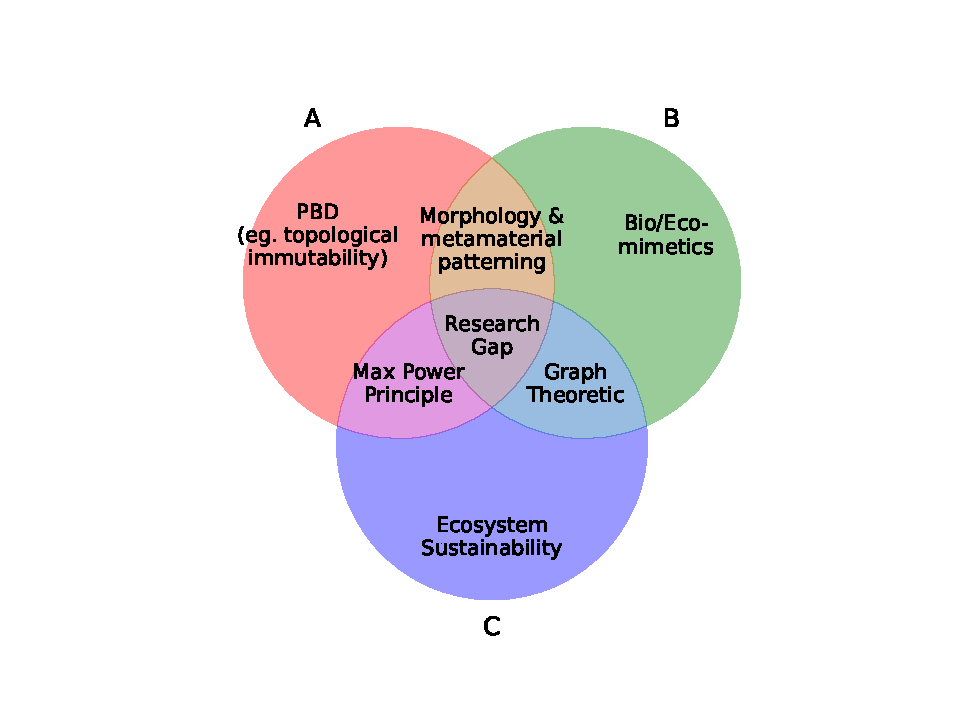
\includegraphics[width=0.7\linewidth]{ven}
    \caption{Venn chart of the interacting conceptual framework used in this thesis.}
    \label{fig:conceptual:framework}
\end{figure}

This chapter is Part A of the literature review. With reference to the conceptual framework given in the Introduction (reproduced in Fig.~\ref{fig:conceptual:framework} for convenience), the present chapter is concerned with the `Eco/Biomimetics' literature, the `Ecosystem Sustainability' literature and the overlap between these domains through the methods of ecological Graph Theoretics. Part B of the literature review is concerned with the concept of `Principle' as a basis of `Principle Based Design' (PBD), and overlaps that PBD has with Ecosystem Sustainability and Eco/Biomimetics. Part B will focus on the \SEs (an ancient type of waterhweel) as a design case for demonstrating the concepts motivating PBD.

Part A of the literature review will begin here by looking briefly at the origins of Biomimetics in the works of \citeauthor{schmitt_biomimetic_1973}. It will then progress to consider the emergence of `Ecomimetics' as an ecological enhancement of Biomimetics introduced in the literature to respond to the criticism that Biomimetics is too reductive. The review will consider how some scholars consider Ecological Engineering, Systems Ecology and Ecological Graphs as integral to Ecomimetics, and in particular the ecological scholarship of Howard T. Odum is identified as a key feature of Ecomimetic literature. The review will therefore consider how the ecological Graph Theoretics of Odum have been suggested as a way of addressing the critique of Biomimetics as reductive. The relationship of Ecosystem Sustainability theory to the Ecomimetics domain will then be introduced through the concepts of Environmental Accounting generated in Odum's scholarship. In so doing the review will also breifly introduce the recent work of \citeauthor{keena_clark_2018} who attempted to develop a novel Grasshopper add-on, `Clark's Crow', which enables the kind of Ecological Accounting analysis of CAD designs envisioned by Odum. Part A will conclude by considering the gaps in the literature as presented here, particularly with reference to the concept of `Principle'. 

\section{Bioimetics}

\begin{quotation}
    ``\textsc{mimetic} 1. Having a particular aptitude for mimicry or imitation; habitually practising imitation or mime.'' \cite{oed_mimetic_2002}
\end{quotation}

In the field of design, the concept of mimetics appears to be most closely associated with the ideas of \citeauthor{schmitt_biomimetic_1973} that reference to the term, ``Biomimetics''. For the purpose of this review, a brief background to \citeauthor{schmitt_biomimetic_1973} concept of Biomimetics will be given with emphasis on three different aspects of \citeauthor{schmitt_biomimetic_1973}'s thinking; `\textit{in the image of life}' (Sec.~\ref{sec:image:life}), `\textit{information transform models}' (Sec.~\ref{sec:information:transform}) and  `\textit{meeting the machine halfway}' (Sec.~\ref{sec:meeting:machine}). 

\subsection{Background to biomimetics}
\label{sec:biomimetics:background}

According to \citet{harkness_appreciation_2002} the concept of Biomimetics originated in the scholarship of the American (Bio-electrical) Engineer Otto Herbert Schmitt (1913-1998 \CE). \citeauthor{harkness_appreciation_2002} says it is uncertain when \citeauthor{schmitt_biomimetic_1973} invented the word ``Biomimetics'', but \citeauthor{harkness_appreciation_2002} locates the first textual appearance in the title of a presentation given \citeauthor{schmitt_biomimetic_1973}, \textit{Some Interesting and Useful Biomimetic Transforms} \cite{schmitt_interesting_1969}.\footnote{The paper was presented at the Third International Biophysics Congress in Boston. The full text of the document appears not to have been recorded in any textually verifiable sources.} In fact, as early as \citeyear{schmitt_signals_1963}, \citeauthor{schmitt_signals_1963} expressed a preference for the word `Biomimetics' over the term `bionics' in his publication, \textit{Signals Assimilable by Living Organisms and by Machines} \cite{schmitt_signals_1963}:\footnote{For \citeauthor{vincent_biomimetics_2006} `Biomimetics' is also synonymous with the words, `biomimesis', `Biomimicry', `biognosis', and with the term `biologically inspired design' \cite[p.~471]{vincent_biomimetics_2006}.}

\begin{figure}[H]
    \centering
    \includegraphics[width=0.6\linewidth]{schmitt_signals_1963_bionics-or-biomimetics_p90.jpg}
    \caption{\cite[p.~90]{schmitt_signals_1963}}
    \label{fig:schmitt:bionics}
\end{figure}

Authors like \citeauthor{bhushan_biomimetics_2009} suggest that the idea of Biomimetics probably arose earlier in \citeauthor{schmitt_biomimetic_1973}'s doctoral research \cite[p.~1445]{bhushan_biomimetics_2009}. To this point, \citeauthor{harkness_appreciation_2002} recounts that \citeauthor{schmitt_biomimetic_1973}'s graduate research was on the general topic of ``biophysical and biochemical methods'' which included the study of the molecular organisation of nerve fibre cells and tissues \cite[p.465]{harkness_appreciation_2002}. But \citeauthor{harkness_appreciation_2002} also says that \citeauthor{schmitt_biomimetic_1973} moved his interest towards the idea of building bioelectric systems rather than just biophysical and biochemical ones, and that this may have been because of \citeauthor{schmitt_biomimetic_1973}'s background in electrical engineering; ``\dots Otto developed a complex electronic device to mimic the generation and propagation of action potentials along nerve fibers'' \cite[p.465]{harkness_appreciation_2002}. It is this aspect of \citeauthor{schmitt_biomimetic_1973}'s research which, I suggest, has been somewhat obscured in contemporary discussions of Biomimetics in relation to design, and will be discussed in Section~\ref{sec:meeting:machine} below. However, the next section will consider the more popular aspect of Biomimetics under the heading, ``\textit{in the image of life}''.

\subsection{\citeauthor{schmitt_biomimetic_1973}'s `In the image of life'}
\label{sec:image:life}

In his \citeyear{schmitt_signals_1963} paper \citeauthor{schmitt_signals_1963} commented that he preferred the word `Biomimetics' over the word `bionics'. This seems to have been partly because for \citeauthor{schmitt_signals_1963} `Biomimetics' was a broader term that not only included the `man-machine systems' of bionics, but also `biological engineering' and `cybernetics' \cite[p.~90]{schmitt_signals_1963}. Using `Biomimetics' as a broader term he expressed what he thought might be the common interests of all these disciplines: 

\begin{figure}[H]
    \centering
    \includegraphics[width=.6\linewidth, frame]{images/schmitt_signals_1963_imageoflife_p90.jpg}
    \caption{\cite[p.~90]{schmitt_signals_1963}}
    \label{fig:schmitt:1963:life}
\end{figure}

The idea of makings things that are, ``in the image of life'', seems to have captured the interests of the secondary literature, where ``Biomimetics'' has been defined as, ``\dots to imitate (mimesis) life (bios) \dots'' \cite[p.54]{kaufmann_biomimetics_2015}. As \citeauthor{ayre_biomimicry_2004} writes, in practical terms Biomimetics is, ``\dots essentially the practice of taking ideas and concepts from nature and implementing them in a field of technology such as engineering, design or computing'' \cite[p.~4]{ayre_biomimicry_2004}. In the examples of Biomimetic research given below, we will see that this idea of mimicking biological systems can be done at many different scales of design, from the molecular to the built environment. 

\subsection{\citeauthor{schmitt_biomimetic_1973}'s information transform model}
\label{sec:information:transform}

A further aspect of \citeauthor{schmitt_signals_1963}'s Biomimetics is the idea of an, ``\textit{information transform model}'' \cite[p.~297]{schmitt_interesting_1969}. The concept of an information transform model doesn't seem to be fully captured by the idea of mimicry given above, but appears to be what \citeauthor{schmitt_signals_1963} also calls ``emulation''. Emulation is ,in \citeauthor{schmitt_signals_1963} terms, the process of building special computers that embody the, ``\dots particular `bio' properties that we want to measure'' \cite[p.~92]{schmitt_signals_1963}. Out of this approach, \citeauthor{schmitt_interesting_1969} suggested that he had developed a ``holographic memory model'' that might assist human pattern recognition. However, at the time he was writing, \citeauthor{schmitt_interesting_1969} noted that he had not yet developed any useful experiments for demonstrating or testing the concept \citep{schmitt_interesting_1969}. 

\subsection{\citeauthor{schmitt_biomimetic_1973} meeting the machine halfway}
\label{sec:meeting:machine}

Another aspect of \citeauthor{schmitt_signals_1963}'s thinking is the idea of, ``meeting the machine halfway'' \cite[p.~91]{schmitt_signals_1963}. As noted above, one of \citeauthor{schmitt_signals_1963}'s intended outcomes of Biomimetics was the potential development of, ``\dots composite bio-physical systems'' \cite[p.~90]{schmitt_signals_1963}. Here \citeauthor{schmitt_signals_1963} appears to be talking about engineering signal systems that might afford novel bio-machine hybrids. But to make these hybrid \citeauthor{schmitt_signals_1963} says we are required to look at three dimensional space, ``\dots for the optimal combinations of man, machinery and the `figures of speech' or the theoretical models'' \cite[p.~91]{schmitt_signals_1963}. \citeauthor{schmitt_signals_1963} gives the following example which pertains to the transfer of three dimensional instruction code to the signal processing of the human brain:

\begin{figure}[H]
    \centering
    \includegraphics[width=.6\linewidth, frame]{images/schmitt_signals_1963_p91.jpg}
    \caption{`Signals into people' \cite[p.~91]{schmitt_signals_1963}}
    \label{fig:schmitt:1963}
\end{figure}

\citeauthor{schmitt_signals_1963} goes on to say that as a part of getting signals into people, ``Surprisingly often a human or two can be built into the machine as an active component at startling savings in cost and with greatly enhanced performance'' \cite[p.~92]{schmitt_signals_1963}.  A human built into a machine is depicted in Figure~\ref{fig:schmitt:human_in_machine}, reproduced from \citeauthor{schmitt_biomimetic_1973}'s paper on \textit{Biomimetic modeling of the heart} \citep{schmitt_biomimetic_1973}.

\begin{figure}[H]
    \centering
    \includegraphics[width=.6\linewidth, frame]{images/schmitt_biomimetic_1973_p487.jpg}
    \caption{`Human in the machine' \cite[p.~487]{schmitt_biomimetic_1973}}
    \label{fig:schmitt:human_in_machine}
\end{figure}

In this way `Biomimetics' seems to have more of the `bionics' meaning, such that the definition is not only talking about copying or mimicking living systems, but also about the engineering of human-machine composites. As mentioned by \citeauthor{ayre_biomimicry_2004}, here \citeauthor{schmitt_signals_1963}'s familiarity with the methods of electric engineering appear to have significance such that the idea of placing humans and life in the bioelectric circuit made them the subject of the mathematical theorems of circuits. This may be why \citeauthor{schmitt_signals_1963} was thinking of a new type of mathematics, and a new type of mathematician:

\begin{figure}[H]
    \centering
    \includegraphics[width=.6\linewidth, frame]{images/schmitt_signals_1963_themathematicians_p91.jpg}
    \caption{`New mathematicians' \cite[p.~91]{schmitt_signals_1963}}
    \label{fig:schmitt:1963:maths}
\end{figure}

To elaborate on this idea \citeauthor{schmitt_signals_1963} refers to one instance where he used stock mathematical treatments in `unconventional combinations'. In doing so he arrived at a ``functional correlation technique''\footnote{This is possibly the `functional analogies' mentioned by \citet{vincent_biomimetics_2006}.} for the analysis of biophysical data. For \citeauthor{schmitt_signals_1963} it appears that the novelty of this technique was not so much that it enabled him to find analogous types, but rather that it required him to treat time as a dependent variable rather than an independent variable.  Describing the utility of this technique \citeauthor{schmitt_signals_1963} says that the activity of varying the time axis gave him, ``\dots new latitude in recognizing what seems biophysically important in electrographic pattern evaluation''  \cite[p.~91]{schmitt_signals_1963}. We shall return to the concept of time as a dependent variable in the discussion of sustainability below. Presently, however, the next section will give some examples of the kind of work that \citeauthor{schmitt_signals_1963}'s ideas have inspired in various domains and scales of fabrication.

\section{Examples of biomimetically inspired designs} 
\label{sec:biomimetic:examples}

\subsection{In the image of life}

\begin{figure}[H]
    \centering
    \includegraphics[width=.8\linewidth, frame]{images/krieg_computational_2012_fig4_shell_p524.jpg}
    \caption{Inspiration: Sand dollar shell \cite[p.~524]{krieg_computational_2012}}
    \label{fig:krieg:2012:shell}
\end{figure}

An example at the scale of the built environment is \citet{krieg_computational_2012}'s case study which took inspiration from the skeletal structure of the sand dollar shell shown in Figure~\ref{fig:krieg:2012:shell}. The mimicry pavilion fabricated by \citeauthor{krieg_computational_2012} is shown in Figure~\ref{fig:krieg:2012:comp}:

\begin{figure}[H]
    \centering
    \includegraphics[width=.8\linewidth, frame]{images/krieg_computational_2012_fig1_p522.jpg}
    \caption{Fabrication: Research pavilion \cite[p.~522]{krieg_computational_2012}}
    \label{fig:krieg:2012:comp}
\end{figure}

The pioneering research of \citeauthor{menges_morphogenesis_2012} has attempted to `up-scale' life's small-scale generative design strategies. Indeed, \citeauthor{menges_morphogenesis_2012} say that biomimetic engineering was the core of their morphogenetic approach to design. In this approach, material (and biological) systems are generative drivers, or forcing functions, of design:

\begin{figure}[H]
    \centering
    \includegraphics[width=.8\linewidth, frame]{images/menges_morphogenesis_2012_biomimetics_p165.jpg}
    \caption{\cite[p.~165]{menges_morphogenesis_2012}}
    \label{fig:menges:morpho}
\end{figure}

Some other examples of the attempt to mimic biological structures in built environment design are, \cite{knippers_design_2012, krieg_computational_2012, erdine_biomimetic_2013, magna_nature_2013, castriotto_biomimetic_2019}. At the small scale, examples of Biomimetics are evident in the work of \citeauthor{parker_biomimetics_2007}, who, for example, were inspired by the anti-reflective properties of moth eye surfaces. \citeauthor{parker_biomimetics_2007} scanned a moth eye shown in Figure~\ref{fig:parker:2007:eye}, and then attempted to mimic the surface by fabrication with ion-beam etching to produce the result depicted in Figure~\ref{fig:parker:2007:replica}.

\begin{figure}[H]
    \centering
    \begin{subfigure}{.45\textwidth}
        \centering
        \includegraphics[width=.95\linewidth, frame]{images/parker_biomimetics_2007_fig1a_b_p348.jpg}
        \caption{Inspiration: Moth eye}
        \label{fig:parker:2007:eye}
    \end{subfigure}
        \hspace{2em}% Space between images
    \begin{subfigure}{.45\textwidth}
        \centering
        \includegraphics[width=.80\linewidth, frame]{images/parker_biomimetics_2007_fig1c_p348.jpg}
        \caption{Fabrication: Moth eye replica}
        \label{fig:parker:2007:replica}    
    \end{subfigure}
    \caption{\cite[Fig.~1a-c, p.~348]{parker_biomimetics_2007}}
\end{figure}

At the micro-scale, researchers have been concerned with the molecular building blocks. A search of ``Nature Reviews'' for example, reveals that the term ``Biomimetics'' has been used across several fields of nanotechnology \citep{sarikaya_molecular_2003, parker_biomimetics_2007}, materials science \citep{ sanchez_biomimetism_2005, hou_interplay_2017}, chemistry \citep{wodrich_natural_2017, levin_biomimetic_2020}, water science \citep{goel_bibliometric_2021}, physics \citep{manna_harnessing_2022}, polymer science \citep{yoshida_development_2010,hirai_microstructured_2019}, dentistry and oral science \citep{pandya_enamel_2019}, smart biomaterials \citep{zhang_advanced_2018}, electronics, microelectronics and microelectromechanical microfabrication \citep{lothman_biomimetic_2014} and even in Information Systems \citep{kaufmann_biomimetics_2015}. 

\subsection{Bio-machine hybrids}

\citeauthor{schmitt_signals_1963}'s idea of Bio-machine hybrids appears to have been taken up from two different perspectives. One approach has been through the idea cyborg and the field of cybernetics, and other is from the perspective of materials science. From the materials science perspective,  \citeauthor{schmitt_signals_1963}, for example, emphasise the hybrid aspect, and has led to the development of a field called ``molecular biomimetics''. As \citeauthor{sarikaya_molecular_2003} wrote,  molecular biomimetics is a, ``\dots marriage of materials science engineering and molecular biology for development of functional hybrid systems'' \cite[p.~579]{sarikaya_molecular_2003}. \citeauthor{sarikaya_molecular_2003} focused on proteins as bio-control structures, under the premise that, ``\dots inorganic surface-specific polypeptides could be used as binding agents to control the organization and specific functions of materials'' \cite[p.~578]{sarikaya_molecular_2003}. Figure~\ref{fig:sarikaya:molecular} is how \citeauthor{sarikaya_molecular_2003} represent the domain of molecular biomimetics as an integration of biology with the synthetic materials from the materials sciences to form genetically engineered and self-assembling materials:

\begin{figure}[H]
    \centering
    \includegraphics[width=.95\linewidth, frame]{images/sarikaya_molecular_2003_Fig2_p579.jpg}
    \caption{Molecular biomimetics \cite[Fig.~2, p.~579]{sarikaya_molecular_2003}}
    \label{fig:sarikaya:molecular}
\end{figure}

But although \citeauthor{sarikaya_molecular_2003} seems to implement a kind of hybrid system, from the bionic perspective of \citeauthor{schmitt_signals_1963}'s bio-machine hybrids, the idea seems to be more concerned with the transfer of a 3D instruction set (perhaps something like G-Code) to a living system, like the human brain. In simple terms the concept appears to view humans like 3D-printers, and as a kind of target system for Computer Aided Manufacturing. To that end, DARPA\footnote{Defense Advanced Research Projects Agency} has researched bio-machine hybrids such as the, ``cyborg beetles''. That is, beetles whose flight is controlled by implanted electrodes and a wireless radio receiver \citep{singer_army_2009} (See Fig.~\ref{fig:singer:darpa}):  

\begin{figure}[H]
    \centering
    \includegraphics[width=.65\linewidth, frame]{images/singer_army_2009_cyborg-beetle.jpg}
    \caption{Bio-machine hybrid beetle \citep{singer_army_2009}}
    \label{fig:singer:darpa}
\end{figure}

\subsection{Emulation and an example from Systems Ecology}

As noted above, \citeauthor{schmitt_signals_1963} himself did not appear to find good experimental examples to demonstrate his concept of emulation and his associated `information transform models'. It is possible, however, to find some discussion of emulators but just not with reference to \citeauthor{schmitt_signals_1963}'s biomimetics. It appears to have required a dialectical paradigm shift away from the `human in the machine' and more toward the `machine in the environment'. The science of Systems Ecology was one domain that appeared to make such a paradigm shift and used the concept of emulation to refer to `microcosms' \cite[p.~187]{beyers_ecological_1993}. \citeauthor{beyers_ecological_1993}, for example, cited \citeauthor{vanvoris_functional_1978}'s depiction of a microcosm as a specific instance of Emulation \cite[p.~238]{beyers_ecological_1993}. \citeauthor{vanvoris_functional_1978}'s depiction is reproduced in Figure~\ref{fig:vanvoris:1978:microcosm}, and presented here as an example of the kind of emulation system that \citeauthor{schmitt_signals_1963} may have been thinking of. 

\begin{figure}[H]
    \centering
    \includegraphics[width=.40\linewidth, frame]{images/vanvoris_functional_1978_fig1_p12.jpg}
    \caption{Microcosm `emulation' \cite[p.~12]{vanvoris_functional_1978}}
    \label{fig:vanvoris:1978:microcosm}
\end{figure}

The intention of \citeauthor{vanvoris_functional_1978} and \citeauthor{beyers_ecological_1993} was to create a small scale ecological system that had all the inputs and outputs controlled so that test conditions could be created to understand the input requirements of the ecological system, and its outputs. This type of ecological mimetics pre-dates the concept of `Ecomimetics', however would seem to apply as a nascent form of Ecomimetics. It is not clear whether the process of creating small ecological systems as emulations led to the development of the concept of Sustainability in the Systems Ecology of  \citeauthor{beyers_ecological_1993}, however, it seems that \citeauthor{schmitt_signals_1963}'s biomimetics does not itself inherently contain a concept of Sustainability, and the next section will briefly introduce critical questions for Biomimetics in this regard.


\subsection{Reductionist criticism of Biomimetics}

\citeauthor{gamage_can_2011} argue that an examination of Biomimicry literature reveals a reductive mindset that makes it difficult to apply the concept, ``\dots as a complete design approach within architecture'' \cite[p.~1]{gamage_can_2011}. The problem with the reductive mindset here is that a design can be considered in and of itself, like a closed system, irrespective to any environmental context. The above presentation of \citeauthor{schmitt_signals_1963}'s Biomimetics and the associated examples of Biomimetic research can be seen to display reductionist characteristics in that they have not explicitly involved the concept of `Sustainability' or transactions with an environment. This is not to say the concept of Sustainability cannot be a key pillar of Biomimetics, but, rather, that Biomimetic designs can be fabricated in the absence of any measure of ecological Sustainability. 

To this point, when reviewing \citeauthor{schmitt_signals_1963}'s original ideas of Biomimetics above, an increase in design sustainability did not appear to be an explicitly intended outcome. For instance, the examples of cybernetic control of beetle flight and the combination of material science and biology in molecular Biomimetics do not present any associated Sustainability metric against which the ``Sustainabilityness'' of the research outcomes might be evaluated. If we consider the Biomimetic pavilion design of \citeauthor{krieg_computational_2012} (Fig.~\ref{fig:krieg:2012:comp}) for example, we can question how the Biomimetic features improve the design Sustainability. Although aesthetically impressive, there does not appear to be any metric that can be used to show how the design was any more or less Sustainable due to its Biomimetic features. The review will now turn to look at the concept of `Ecomimetics' which has been introduced in response to this criticism. It will also consider the `Graph Theoretic' implications of the Ecomimetic approach as it is used by \cite{holguera_ecomimetics_2014} and \cite{garcia-holguera_ecomimetics_2018}.

\subsection{The Ecomimetics response}

In response to the reductionist criticism of Biomimetics, some scholars like \citeauthor{gamage_can_2011} argue for an ``ecological Biomimetics'' which they call ``Ecomimetics''. Ecomimetics, say \citeauthor{gamage_can_2011}, is based on a holistic view of Biomimicry that, ``\dots goes beyond mimicking a particular organism, process or ecosystem'' \cite[p.~1]{gamage_can_2011}. The aim of this kind of holism is to situate a design in an environmental context. A design, then, is as an open system which seeks to understand the inputs and outputs between a design and its environment. As a part of this holistic view a design is understood to be dynamic and transformed by its environment, but also transforming its environment through exchanges of matter, energy and information. \citeauthor{gamage_can_2011} anticipate that such a holistic Ecomimetic design philosophy might start a design revolution for many disciplines, ``\dots based on principles of ecology that studies the relationship of flora and fauna'' \cite[p.~2]{gamage_can_2011}. 

It is noteworthy here that \citeauthor{gamage_can_2011} don't elaborate on the definition of the word `Principle', nor how it might be related to ecological systems, ecological Biomimetics or Sustainable design. Nevertheless, for \citeauthor{gamage_can_2011}, an Ecomimetic design philosophy would need to integrate ecological ideas that view nature's adaptation and integration strategies as transformations \cite[p.~1]{gamage_can_2011}. Indeed, \citeauthor{gamage_can_2011}'s focus on nature's transformation strategies here seems to partly align with \citeauthor{schmitt_signals_1963}'s concept of `information transformation models'. 

\citeauthor{holguera_ecomimetics_2014} has presented theoretical outlines for an Ecomimetic methodology \citep{garcia-holguera_ecosystems_2013, holguera_ecomimetics_2014, garcia-holguera_ecomimetics_2018}. For \citeauthor{holguera_ecomimetics_2014} Ecomimetics and the Ecomimetic methodology uses concepts and tools from several disciplines in the attempt to, ``\dots build bridges between ecosystems and building design'' \citep[p.4]{holguera_ecomimetics_2014}. But in taking this approach \citeauthor{holguera_ecomimetics_2014} direct attention to the often-observed problem of ecological complexity which arises through holistic methods. \citeauthor{holguera_ecomimetics_2014} make note of authors like \cite{bertalanffy_outline_2008}, \cite{barabasi_emergence_1999} and \cite{anand_ecological_2010} who have developed General Systems Theory and Graph Theoretic methods that attempt to accommodate the challenges presented by ecological network complexity. And in addition to these methods \citeauthor{holguera_ecomimetics_2014} makes an appeal to the identification of general principles and feedback loops as important features that need to be accommodated in Ecomimetic design practice: 

\begin{figure}[H]
    \centering
    \includegraphics[width=.95\linewidth, frame]{images/holguera_ecomimetics_2014_p4.jpg}
    \caption{\cite[p.~4]{holguera_ecomimetics_2014}}
    \label{fig:holguera:Ecomimetics}
\end{figure}

Earlier, \citeauthor{garcia-holguera_ecosystems_2013} identified Ecological Engineering as a key discipline that may have methods to assist Ecomimetic design with the problems posed by ecological network complexity. They cite the scholarship of \citeauthor{mitsch_ecological_1989} together with \citeauthor{odum_ecological_1994} as key works involved in the development of tools that attempted to integrate qualitative with quantitative approaches to ecological complexity. For instance, \citeauthor{garcia-holguera_ecosystems_2013} bring specific attention to \citeauthor{odum_ecological_1994}'s diagramming method known as the `Energy Systems Language'.\footnote{\citeauthor{holguera_ecomimetics_2014} refer to \citeauthor{odum_ecological_1994}'s qualitative tool as Energy System Diagrams. \citeauthor{odum_ecological_1994}, however, referred to it by various names such as Energy Circuit Language, Energy Systems Language and \textit{Energese}. It will be referred to here as the `Energy Systems Language'.} One of \citeauthor{odum_ecological_1994}'s early descriptions of the language is given below (Fig.~\ref{fig:odum:tropical}):

\begin{figure}[H]
    \centering
    \includegraphics[width=.55\linewidth, frame]{images/odum_tropical_1970a_pA6.jpg}
    \caption{\cite[p.~A6]{odum_tropical_1970a}}
    \label{fig:odum:tropical}
\end{figure}

\citeauthor{odum_energy_1972}'s Energy Systems Language was developed to afford the comprehension of ecological network complexity by a method of systematically arranging qualitative ecological concepts captured in the symbols of the langauge (Fig.~\ref{fig:odum:tropical}) into schematic-like graphs.\footnote{See \citet[pp.A5-A11]{odum_tropical_1970a} and \citet[pp.~139–211]{odum_energy_1972}.} The purpose of the ecological graphs was to subsequently afford designers to generate a quantitative simulation of the energy flows, storages, and limiting-factors in an ecosystem. A further description of the use of these symbols and language will be given in the Thesis methodology section, however, as an introduction, the key symbols of the Energy Systems Language are depicted in Figure~\ref{fig:odum:tropical} with an example of their usage in Figure~\ref{fig:srinivasan:re}:

\begin{figure}[H]
    \centering
    \includegraphics[width=.5\linewidth, frame]{images/odum_tropical_1970_Fig1_pA6.jpg}
    \caption{Key symbols for the Energy Systems Language \cite[p.~A6]{odum_tropical_1970a}}
    \label{fig:odum:tropical}
\end{figure}

\citeauthor{holguera_ecomimetics_2014} note that \cite{odum_material_2003} attempted to pioneer the application of his ecological schematics to the discipline of Design, and that this effort has been continued by \cite{srinivasan_redefining_2012}. In Figure~\ref{fig:srinivasan:re}, for example, \citeauthor{srinivasan_redefining_2012} use the Energy Systems Language to depict all the inflows and outflows between a building design and its environment. 

\begin{figure}[H]
    \centering
    \includegraphics[width=.65\linewidth, frame]{images/srinivasan_re_2012_Fig3_p304.jpg}
    \caption{Diagram of building environmental design showing energy pathways \cite[Fig.~3, p.~304]{srinivasan_redefining_2012}}
    \label{fig:srinivasan:re}
\end{figure}


\citeauthor{holguera_ecomimetics_2014} themselves in \citeyear{garcia-holguera_ecosystems_2013} produced an ecological graph of a passive solar family house in Hudson (USA) using the Energy Sysetms Language (Fig.~\ref{fig:garcia:hudson}):

\begin{figure}[H]
    \centering
    \includegraphics[width=.7\linewidth, frame]{images/garcia-holguera_ecosystems_2013_Fig4.jpg}
    \caption{Ecological graph of passive solar family house \cite[Fig.~4]{garcia-holguera_ecosystems_2013}}
    \label{fig:garcia:hudson}
\end{figure}

A further example that might be more graphically illustrative is the work of \citeauthor{keena_visualization_2016} who has attempted to apply the Energy Systems Language method but using more qualitative pictograms and graphic design to visualise the Ecological inputs into the Farnsworth house \citep{keena_visualization_2016} as shown in Figure~\ref{fig:farnsworth}: 

\begin{figure}[H]
    \centering
    \includegraphics[width=0.5\linewidth]{images/keena_2016_ESLFarnsworth_Fig4_p134.jpg}
    \caption{Ecological graph visualisation of Farnsworth house by \citet[Fig.~4, p.~134]{keena_visualization_2016}.}
    \label{fig:farnsworth}
\end{figure}

\subsection{Summary of Ecomimetics}

In all of the examples of using the graph theoretic method of \citeauthor{odum_ecological_1994} to generate holistic concepts of design, a number of quesions and issues seem to remain. For while the concept of Ecomimetics has arisen out of the attempt to make Biomimetics holistic in scope, and despite the efforts of \citeauthor{srinivasan_hierarchy_2015}, the graph theoretic methods of \citeauthor{odum_ecological_1994} do not appear to have been used widely as a part of design methods. Part of the evidence for this assertion is that although \citeauthor{odum_simulation_1989} has given several computational examples for the Energy Systems Language method \citep{odum_energy_1972, odum_simulation_1989, odum_ecological_1994}, the key symbols and simulation methods have not been integrated into commonly used Computer Aided Design tools like Rhino3D and Grasshopper. And even although \citeauthor{holguera_ecomimetics_2014} have sought to integrate the methods of Ecological Engineering the question of how to evaluate the Sustainability of an `ecological Biomimetic' design using the Energy Systems Language still remains opaque. How, for instance, do \citeauthor{odum_ecological_1994}'s diagrammatic methods show ecological Biomimetic designers the Sustainability of their design? These questions motivate the next section which will review how the Ecosystems Engineering literature has attempted to provide answers.

\section{Sustainability}

Before we consider how the Ecomimetic use of \citeauthor{odum_ecological_1994}'s graph theoretic methods might enable an evaluation of a design's Sustainability, we will first consider the definition of terms. Unfortunately, however, it is difficult to provide a canonical definition for the word \textsc{sustainability}. The OED gives three distinct origins all formed within English by derivation; 1. A legal origin pertaining to the, ``\dots quality of being sustainable by argument; the capacity to be upheld or defended as valid, correct, or true'', 2. An economic context pertaining to the longevity of economic growth, and 3. An environmental context relating to, ``\dots the degree to which a process or enterprise is able to be maintained or continued while avoiding the long-term depletion of natural resources'' \cite{oed_sustainability_2022}. Whilst the idea of sustainability referred to in this thesis is most closely aligned with the third definition, it should also be acknowledged that even within the environmentally oriented scholarship the concept means different things to different scholars. This is partly because there has not been a universally agreed upon metric for the evaluation of a design's sustainability.


\subsection{Ecosystem Sustainability}

The discussion that is of most interest is that arising out of what will be identified as the `Florida School'.\footnote{For a root-branch depiction of the lineage of those scholars associated with the Florida School, see the fronticepiece of \citeauthor{hall_maximum_1995}'s Festschrift for Howard T Odum \cite{hall_maximum_1995}.} Although several branches of scholarship emerged from the Florida School, it has been the work around the sustainability indices and bookkeeping methods which has been most developed, and yet, as \citeauthor{gronlund_why_2019} has observed, has also been the most difficult to communicate.

In \citeyear{ulgiati_emergy_1994}, \citeauthor{ulgiati_emergy_1994} attempted to comunicate a definition of Sustainability with respects to the Environmental Accounting paradigm they were developing as a part of the holistic methods of Systems Ecology and Ecological Engineering emerging from the Florida School:

\begin{figure}[H]
    \centering
    \includegraphics[width=.8\linewidth, frame]{images/ulgiati_emergy_1994_p215.jpg}
    \caption{\citet[p.~215]{ulgiati_emergy_1994} on long-term sustainability}
    \label{fig:srinivasan:re}
\end{figure}

The key idea that will be emphasised here is that of an environment\footnote{Following \citet{odum_ecological_1994} the word `environment' will be used interchangeably with the word `ecosystem' without loss of meaning.} `sustaining transformations' for some duration of stability. In a design context, the question of defining Sustainability seems to be one of an environment's design-affordance.  \citeauthor{gronlund_why_2019} attempted to communicate this idea of environment's design-affordance with reference to the concept of a hierarchical `triple-bottom-line', and \citet[Fig.~3, p.~41]{gronlund_why_2019} then used the Energy Systems Language to depict such (Fig.~\ref{fig:gronlund:why}):

\begin{figure}[H]
    \centering
    \includegraphics[width=.95\linewidth, frame]{images/gronlund_why_2019_fig3_p41.jpg}
    \caption{Triple-bottom-line in the energy hierarchy \citet[Fig.~3, p.~41]{gronlund_why_2019}}
    \label{fig:gronlund:why}
\end{figure}

We can see that on the left-hand side of Figure~\ref{fig:gronlund:why}, \citeauthor{gronlund_why_2019} uses a green box to ring-fence the concept of ecological sustainability. \citeauthor{gronlund_why_2019} does this to show that the ecological system make a contribution to the economic system (the blue box), which in turn makes a contribution of information and services to the social system (the red box). It is in this sense that the ecosystem affords certain economic designs, and an economy affords certain social designs. One question for a designer of artefacts here, is whether their design matches the affordances of the ecosystem inputs, and the material cycle that the design and the design fabrication processes feedback to the ecological system. This material cycle feedback from the economy of design fabrication is depicted by \citeauthor{gronlund_why_2019} in Figure~\ref{fig:gronlund:why} with arrows that exit from the bottom of the blue box and return around through the red box to circle back around above the blue box back to the ocean and land of the ecosystem. 



% One of the ideas here is that Ecomimetics, adopts one of the tenets of the Ecosystems Engineering which is that often the longevity, or sustainability, of a design is a question of what designs the environment can afford. Design is about environmental affordances. 


% ``Many principles of ecology have been better illustrated in a microcosm than in the greater, global outdoors. While leaving out some phenomena, miniaturization has allowed organizational phenomena, normally requiring years, to show up in months.'' \cite[p.~433]{beyers_ecological_1993}. 


% This approach attempts to represent information and energy transformation circuits of ecological networks with various schematic and diagrammatic systems, and in this way seems to have a connection with \citeauthor{schmitt_biomimetic_1973}'s `information transformation models'. And further, \citeauthor{schmitt_biomimetic_1973}'s concepts about meeting the machine in the middle as shown in Figure~\ref{fig:schmitt:human_in_machine} depicts a human embedded within the electrical circuits of a machine. These circuits can be represented in Graph Theoretic terms, and so it seems that \citeauthor{schmitt_biomimetic_1973}'s ideas are, at least, not alien to \citeauthor{holguera_ecomimetics_2014}'s formulation of Ecomimetic design philosophy, if not necessitated it. 



% With this acknowledgement, the branch of sustainability theory that is of interest to thesis arises due to the 


\subsection{Clark's Crow and Total Environmental Accounting}

Although it was noted above that \citeauthor{odum_ecological_1994}'s Energy Systems Language and methods had not been integrated into popular CAD packages, there has been an attempt to integrate the accounting methodology of the Florida School into Grasshopper. In the period leading up to their \citeyear{keena_clark_2018} paper for instance, \citeauthor{keena_clark_2018} developed a novel Grasshopper add-on for the Rhinocerous 3D CAD software package. \citeauthor{keena_clark_2018} called their add-on `Clark's Crow' (Fig.~\ref{fig:clarkscrow}), and described it as a tool that could be used during the design decision-making process to evaluate the socio-ecological impact of different design options \cite[pp.~42-44]{keena_clark_2018}. In the development of `Clark's Crow' \citeauthor{keena_clark_2018} leveraged the existing Grasshopper add-on called `Ladybug'\footnote{See \cite{ladybug_ladybug_2016}}, which in turn uses `Honeybee'\footnote{See \cite{ladybug_honeybee_2022}}, to import OpenData on energy for the modelling and analysis of designs (See also Fig.~\ref{fig:clarkscrow:workflow}). 

\begin{figure}[H]
    \centering
    \includegraphics[width=0.55\linewidth]{images/keena_2018_clarkscrowaddin_p46.jpg}
    \caption{Clark's Crow Grasshopper Add-in \cite[p.~46]{keena_clark_2018}.}
    \label{fig:clarkscrow}
\end{figure}

The intention of using `Honeybee' and `Ladybug' was to enable `Clark's Crow' users to evaluate the sustainability of their design by accounting for all the energy flows, starting with energy flows into the geo-biosphere from the sun. The novelty here is the (attempted) implementation of an ecological accounting method known as `emergy evaluation'. The word `emergy', spelled with an `m', is a shorthand for the term `embodied energy', and is used specifically to refer to a distinctive ecological accounting approach pioneered by \citet{odum_environmental_1996}.\footnote{The emergy nomenclature (the words, method and terms used together with the word `emergy') was developed by Odum, his students and colleagues---especially an Australian fellow by the name of David Scienceman---which is what I'm referring to collectively as the `Florida School'.}

\begin{figure}[H]
    \centering
    \includegraphics[width=0.98\linewidth]{images/keena_2019_clarksCrow_Fig1_p61.jpg}
    \caption{\citeauthor{keena_benefit_2019} \citeyearpar[Fig.~1, p.~61]{keena_benefit_2019} visualising an integration of Environmental Accounting and Grasshopper.}
    \label{fig:clarkscrow:workflow}
\end{figure}

The accounting method behind the emergy nomenclature was intended to be holistic in scope, which means that it aimed track all the potential and actual inputs into a system design using the energy available from sunlight hitting the geo-biosphere as a common base unit.\footnote{This unit is referred to as the `solar emergy joule', or `semj'. However in the tradition of using surnames to refer to a scientific unit the `Odum' might be a better way to refer to the solar emergy joule as a common base unit.} In Figure \ref{fig:holistic} \citeauthor{keena_clark_2018} depicted the holistic scope of the emergy method in contrast with other life cycle analysis methods which operate on a restricted part of the system as a whole.

\begin{figure}[h!]
    \centering
    \includegraphics[width=0.85\linewidth]{images/keena_2018_giobiosphere_p43.jpg}
    \caption{Relationship of different accounting methods compared to holistic `whole of system'  emergy method \cite[p.~43]{keena_clark_2018}.}
    \label{fig:holistic}
\end{figure}

According to \citeauthor{keena_clark_2018} the Honeybee Grasshopper add-on in particular includes many of the prerequisites required for the calculation of the emergy values detailed in \citeauthor{odum_environmental_1996}'s book, and was therefore leveraged in the development of Clark's Crow. An example of the novelty provided by Clark's Crow, prior to its development researchers like \cite{tabony_ecological_2021} used the Systems Dynamics\footnote{See \cite{forrester_principles_1999}} simulation platform called STELLA for the task of modelling sustainability of Urban Design. However, at the time of writing, the STELLA software package was not integrated with Rhinocerous 3D/Grasshopper. Furthermore, the STELLA software uses hydraulic analogies based on stock-flow algorithms \cite[p.~100, Fig.~3.43]{tabony_ecological_2021} which seems to have meant that \citeauthor{tabony_ecological_2021} was unable to use the `track-summing'\footnote{For mathematical treatments of the track-summing methods see the discussion in; \cite{tennenbaum_network_1988, tennenbaum_emergy_2015, tennenbaum_odumtennenbaumbrown_2015, le_corre_odumtennenbaumbrown_2015}.} process of the emergy method in the simulation of system designs. Hence Clark's Crow was novel both in the use of the emergy method and in the integration with Grasshopper, and with further feature enhancement may be able to replace the STELLA product in the simulation of system designs in Rhino 3D.

\citeauthor{keena_clark_2018}'s development of Clark's Crow is of interest in this thesis because, not only is it another attempt\footnote{See for example \cite{valyi_user_2005, valyi_emergy_2004-4, valyi_emergy_2004-3, valyi_emergy_2004-2, valyi_emergy_2004, valyi_emergy_2004-1}, and Extend\texttrademark  shown in \cite{odum_modeling_2000}.} to build a tool to facilitate the somtimes controversial\footnote{See, for example, the commentary in \citeathor{valyi_user_2005}' thesis. See also the discussion in \cite{baktari_emergy_2000, tennenbaum_network_1988, tennenbaum_emergy_2015, le_corre_odumtennenbaumbrown_2015, tennenbaum_odumtennenbaumbrown_2015}.} ecological accounting method of \cite{odum_environmental_1996}, but also because it aims to relate the output of Computer Aided Design with the ``life cycle'' requirements of the design and its materials, including the scale of Earth's geo-biosphere. As \cite{keena_clark_2018} write:

\begin{quotation}
    ``How we process, recover, restore and regenerate both the technical “nutrients” of the techno-sphere and the biological nutrients of the geo-biosphere within urban ecosystems is thus a crucial question when considering sustainable urban development.'' \cite[p.~42]{keena_clark_2018}
\end{quotation}

The adoption of \cite{odum_environmental_1996}'s accounting method by \citeauthor{keena_clark_2018} is also of interest here because of a prevailing gap in this type of analysis. 

\section{Gaps}

\textsc{to appear}

% The gap becomes evident on a closer inspection of \citeauthor{odum_environmental_1996}'s overarching project. \citeauthor{odum_environmental_1996}'s project might be characterised by four main pillars: i) a Generic Energy Systems Language for creating energy systems and circuit diagrams; ii) an accounting method that tracked all inputs and outputs of an ecological economic system; iii) the simulation modelling of hierarchical feedback controls exercised by `quality upgraded' components operating as metabolic energy transformers; iv) an evolutionary `principle' that seeks to maximise the rate of useful energy transformation, where `useful' refers to the generation of sustainable systems. Figure~\ref{fig:odumproject} depicts these four pillars in a diagram.

% It is unclear whether i-iv is required to achieve sustainable and human designed systems, or whether they can be achieved by other means. Nevertheless, it can be observed that in building `Clark's Crow' \citeauthor{keena_clark_2018} appear to have attempted to encode pillars i-iii. A gap here, however, seems to be the absence of pillar iv, and it is this gap that the thesis is concerned to address. Pillar iv is concerned with sustainbility and selective advantage that some designs have over others. Odum considered that it originated in the works of Podolinksky, Lotka, Boltzmann and others and was used as a means of explaining the `persistence of stable forms', that is the sustainability of those forms.

% ``Pre-existing Grasshopper plug-ins targeted at urban studies include Ladybug (Roudsari et al., 2013) for climate analysis and Honeybee (Roudsari et al., 2014) for operational energy and daylight considerations.''

% leverages the EnergyPlus Materials Library from HoneyBee and the Rhino 3D urban model geometry \citeyearpar[p.~47]{keena_clark_2018}, and 




\section{Summary}

\textsc{to appear}


% The ideas of \citeauthor{menges_morphogenesis_2012} 

% In this way design itself appears to be an emergent property of the system fabrication, rather than something applied, top-down by a pre-fabrication human activity. This concept seems to be 



% \citeauthor{menges_morphogenesis_2012}

% theories of self-organising systems to structural design, form finding and research on physical materials

% theory, performativeness is the quality of material systems that perform through deformation, or which visibly deform to self-organise and resist new external forces (loads,for example).



% One of the tools that scholars have used haphazardly is what \citeauthor{}





% The second is the absence of the `Energy Systems Language' (\textit{Energese}) which was a diagramming language with a syntax and was commonly used pedagogically to communicate the ideas of multiple scales and hierarchical energy flows that typically operate in ecosystems, and whose relevance to Architectural design has been identified by \cite{srinivasan_hierarchy_2015}. 

% Both of these gaps were defining features of the emergy paradigm practised by the Florida School. The chapter will then conclude with the approach proposed in this thesis to fill these gaps, firstly by abstracting the concept of a `Maximum Power Principle' into a broader idea of `Principle-Based Design', which will be demonstrated through by fabricating \SEs with 3D printers as a design case, and secondly by looking at the enhancing `Clark's Crow' to enable the kind of diagrams given by \cite{keena_visualization_2016} to depict the energetics of the Farnsworth house (Shown in Fig.~\ref{fig:farnsworth})


% is thesis 



% Writing in the \textit{Ecological Modelling} journal in \citeyear{ulgiati_emergy_1994}, \citeauthor{ulgiati_emergy_1994} 


% \begin{figure}[H]
%     \centering
%     \includegraphics[width=.65\linewidth, frame]{images/ulgiati_emergy_1994_p215.jpg}
%     \caption{\cite[p.~215]{ulgiati_emergy_1994}}
%     \label{fig:vanvoris:1978:microcosm}
% \end{figure}



% \textit{International Journal of Energy Research}, \citeauthor{hammond_energy_2007} 








% Part A is concerned to look at contemporary concepts of sustainable design from the points of view of overlapping 


% It is made up from two different strands of investigation into contemporary literature regarding the motivation of this thesis. Firstly is ecological and ecobiomimetic motivation. Secondly is a motivation regarding the design and analysis of the \SE. 

% For the former, the review will look at recent work by \citeauthor{keena_clark_2018} 





%  The chapter will introduce both `Clark's Crow' together with six key features Howard T. Odum\footnote{Odum was considered by some to be the `father' of System Ecology and the `ecosystem' concept. The body of work generated by Odum, his students and colleagues might be loosely identified as the `Florida School'.} ``emergy'' project. The chapter will provide a definition of the ``emergy'' concept and identify gaps in `Clark's Crow' system and associated contemporary literature when compared with Odum's project (See Figure~\ref{fig:features}). It will then conclude by proposing some ways to fill the gaps by introducing the concept of Principle-Based Design that can be demonstrated with reference to the \SEs, an ancient type of water wheel. This in turn necessitates a second, historial, literature review regarding the \SEs and the concept of `Principle' arising from early modern Cartesian scholarship. This second literature review will be undertaken in Chapter 3b.

% \section{Gaps}

% The first gap is the absence of a focus on the role of functional analogies used in the General Systems community to formulate the mathematics of components used in a simulation model. This gap is important because it introduces a procedural workflow for transdisciplinary thinking, such that it seeks to generalise concepts which can help transfer mathematics between intellectual domains. Another gap is the absence of the Maximum Power Principle which was identified as relevant to sustainability design workflows in the 

% The second gap is the absence of the `Energy Systems Language' (ESL, also called `\textit{Energese}') which was identified by \cite{srinivasan_hierarchy_2015} as relevant to the depiction of sustainable Urban designs. ESL is a diagramming language developed by Odum during Radiation Ecology studies with a syntax based on `energy-types', and was commonly used pedagogically to communicate the ideas of multiple scales and hierarchical energy flows that typically operate in ecosystems. Although \citeauthor{keena_visualization_2016} visualised the Farnsworth house using a pictorially enhance version of Odum's Energy Systems Language (shown in Figure~\ref{fig:farnsworth}) it was not proposed as a feature of the Clark's Crow tool. 

% \begin{tabular}{p{0.35\linewidth} | p{0.6\linewidth}}
%     odum_1970_envpowsoc_Fig2-5_p40
%     \includegraphics[width=0.99\linewidth]{images/odum_1975_circuit_marine_Fig6-4_p131.jpg}
% \begin{table}[h!]
%     \small 
%     \centering
%     \begin{tabular}{p{0.15\linewidth}|p{0.40\linewidth}|p{0.40\linewidth}} 
%         Feature & \citeauthor{odum_ecological_1994} & \citeauthor{keena_visualization_2016} \\
%         \hline
%         Energy Systems Language & \includegraphics[width=0.59\linewidth]{images/odum_1970_envpowsoc_Fig2-5_p40.jpg} & \includegraphics[width=0.79\linewidth]{images/keena_2016_ESLFarnsworth_Fig4_p134.jpg} \\	
%         Energy Hierarchy &  & \\	
%         Model-Based System Engineering and Simulation & \includegraphics[width=0.79\linewidth]{images/odum_2000_modeling_figP1_pxvii.jpg} & \\	
%         Maximum Power Principle & \includegraphics[width=0.79\linewidth]{images/costanza_introduction_2014_fig2-9_p70.jpg} & \\	
%     \end{tabular}
%     \caption{Comparison of paradigms; Florida School vs Clark's Crow}
%     \label{tab:arithmetic}
% \end{table}

% \begin{sidewaysfigure}[ht]
%     \includegraphics[width=\textwidth]{images/odum_pillars.jpg}
%     \caption{Six key features of Odum's project contrasted with the Clark's Crow Grasshopper Add-on.}
%     \label{fig:pillars}
% \end{sidewaysfigure}

% \begin{landscape}
% \begin{figure}[h!]
%     \centering
%     \includegraphics[width=\linewidth]{images/odum_pillars.jpg}
%     \caption{Six key features of Odum's project contrasted with the Clark's Crow Grasshopper Add-on.}
%     \label{fig:features}
% \end{figure}
% \end{landscape}

% \begin{figure}[h!]
%     \centering
%     \includegraphics[width=\linewidth]{images/odum_pillars.jpg}

%     \label{fig:holistic}
% \end{figure}




\bibliography{MyLibrary}

\printbibliography

\end{document}